\documentclass{article}

\usepackage{ifthen}
\newif\ifsolutions
\solutionsfalse

\usepackage{xcolor}
\usepackage{titleps}
\usepackage[letterpaper, margin=0.95in]{geometry}
\usepackage{url}
\usepackage{amsmath}
\usepackage{amsfonts}
\usepackage{amssymb}
\usepackage{wrapfig}
\usepackage{float}
\usepackage{mathtools}
\usepackage{enumitem}
\usepackage{tabu}
\usepackage{parskip}
\usepackage{natbib}
\usepackage{listings}
\usepackage{tcolorbox}
\usepackage{forest}
\usepackage{hyperref}
\usepackage[color=red]{todonotes}
\usepackage{forest}
\definecolor{light-yellow}{HTML}{FFE5CC}
\usepackage{cleveref}
\usepackage[linesnumbered,ruled,vlined]{algorithm2e}
\usepackage{kotex}
\usepackage{graphics}
\crefname{algorithm}{Algorithm}{Algorithms}
\Crefname{algorithm}{Algorithm}{Algorithms}

\newcommand{\xb}{\mathbf{x}}
\newcommand{\yb}{\mathbf{y}}
\newcommand{\wb}{\mathbf{w}}
\newcommand{\Xb}{\mathbf{X}}
\newcommand{\Yb}{\mathbf{Y}}
\newcommand{\tr}{^T}
\newcommand{\hb}{\mathbf{h}}
\newcommand{\Hb}{\mathbf{H}}

\DeclareFontShape{OT1}{cmtt}{bx}{n}{<5><6><7><8><9><10><10.95><12><14.4><17.28><20.74><24.88>cmttb10}{}

\newpagestyle{ruled}
{\sethead{Berkeley CS 285}{Deep Reinforcement Learning, Decision Making, and Control}{Chanjoon Park}\headrule
  \setfoot{}{\ifsolutions\LARGE\bf\textcolor{red}{Answer Key}\fi}{}}
\pagestyle{ruled}

\renewcommand\makeheadrule{\color{black}\rule[-.75\baselineskip]{\linewidth}{0.4pt}}
\renewcommand*\footnoterule{}

\tcbset{
  answerbox/.style={
    colback=white,
    colframe=black!30,
    fonttitle=\bfseries,
    coltitle=black,
    title=Answer,
    boxrule=0.5pt,
    arc=4pt,
    left=6pt,
    right=6pt,
    top=4pt,
    bottom=4pt,
    before skip=8pt,
    after skip=8pt,
    parskip=12pt
  }
}

\begin{document}
\lstset{basicstyle = \ttfamily,columns=fullflexible,
% backgroundcolor = \color{light-yellow},
breaklines = true,
frame = single,
language = bash
}

\begin{centering}
    {\Large Assignment 3: Q-Learning and Actor-Critic Algorithms} \\
    \vspace{.25cm}
    \textbf{27th March 2025} \\
\end{centering}

\section{Multistep Q-Learning}

\begingroup
\def\Q{Q_{\phi_k}}
\def\Qn{Q_{\phi_{k+1}}}
\def\D{\mathcal{D}}

Consider the $N$-step variant of Q-learning described in lecture. We learn $\Qn$ with the following updates:\begin{align}
  y_{j,t} &\gets \biggl(\;\sum_{t'=t}^{t+N-1} \gamma^{t'-t} r_{j,t'}\biggr)+\gamma^{N} \max _{\mathbf{a}_{j,t+N}} \Q\left(\mathbf{s}_{j,t+N}, \mathbf{a}_{j,t+N}\right) \label{eq:q_target}\\
  \phi_{k+1} &\gets \underset{\phi\in\Phi}{\arg\min}  \sum_{j,t} \bigl( y_{j,t}-Q_{\phi}(\mathbf s_{j,t},\mathbf a_{j,t}) \bigr)^2 \label{eq:q_update}
\end{align}
In these equations, $j$ indicates an index in the replay buffer of trajectories $\D_k$. We first roll out a batch of $B$ trajectories to update $\D_k$ and compute the target values in \eqref{eq:q_target}. We then fit $\Qn$ to these target values with \eqref{eq:q_update}. 
After estimating $\Qn$, we can then update the policy through an argmax:\begin{align}
  \pi_{k+1}\left(\mathbf{a}_{t} \mid \mathbf{s}_{t}\right)\gets \left\{\begin{array}{l}1 \text { if } \mathbf{a}_{t}=\arg \max _{\mathbf{a}_{t}} Q_{\phi_{k+1}}\left(\mathbf{s}_{t}, \mathbf{a}_{t}\right) \\ 0 \text{ otherwise. }\end{array}\right. \label{eq:policy_improvement}
\end{align}
We repeat the steps in \cref{eq:q_target,eq:q_update,eq:policy_improvement} $K$ times to improve the policy. In this question, you will analyze some properties of this algorithm, which is summarized in \Cref{alg:multi}.

\begin{algorithm}[H]
  \caption{Multistep Q-Learning}
  \label{alg:multi}
  \KwIn{Iterations $K$, batch size $B$}
  Initialize random policy $\pi_0$, sample $\phi_0 \sim \Phi$\;
  \For{$k \gets 0$ \KwTo $K-1$}{
      Update $\mathcal{D}_{k+1}$ with $B$ new rollouts from $\pi_k$\;
      Compute targets with~\eqref{eq:q_target}\;
      $Q_{\phi_{k+1}} \gets$ update with~\eqref{eq:q_update}\;
      $\pi_{k+1} \gets$ update with~\eqref{eq:policy_improvement}\;
  }
  \Return $\pi_K$\;
\end{algorithm}


\def\makecols#1#2{{\def\p{#2}\newcount\i\i0\hfill\loop\advance\i1\makebox[1cm][c]{\expandafter\p\the\i}\kern.5cm\ifnum\i<#1\repeat\kern-1cm}}
\def\heading#1{\bf\expandafter\uppercase\expandafter{\romannumeral#1.}}
\def\boxes#1{\ensuremath\square}
\def\filled#1#2|#3{\ifnum#1=#3\ensuremath\blacksquare
	\else\if\relax#2\relax\ensuremath\square
	\else\filled#2|#3\fi\fi}
\def\ncol{3}
\newcommand{\checkeditem}[2]{\edef\x{0#1}\item[\expandafter\filled\x|#2]}


\def\choices#1#2{
	\begin{enumerate}
	\item on-policy in tabular setting \makecols\ncol{\filled0#1|}
	\item off-policy in tabular setting \makecols\ncol{\filled0#2|}
	\end{enumerate}
}

\subsection{TD-Learning Bias (2 points)}
\label{q:td_bias}

\def\answer{2} % <--- TODO: insert index (0/1) of answer
\ifsolutions\solve\thesubsection\fi
We say an estimator $f_\D$ of $f$ constructed using data $\D$ sampled from process $P$ is \textit{unbiased} when $\mathbb{E}_{\D\sim P}[f_\D(x)-f(x)]=0$ at each $x$.

Assume $\hat Q$ is a noisy (but unbiased) estimate for $Q$. Is the Bellman backup $\mathcal{B}\hat Q = r(s, a) + \gamma \max_{a'} \hat Q(s', a')$ an unbiased estimate of $\mathcal{B}Q$?
\begin{itemize}
    \checkeditem\answer1 Yes
    \checkeditem\answer2 No
\end{itemize}

\begin{tcolorbox}[answerbox, parbox=false]
  An unbiased estimator is expected value equals the true value. $\mathbb{E}[\mathcal{B}\hat{\mathcal{Q}}] = \mathcal{BQ}$. so, $\mathbb{E}[\mathcal{B}\mathcal{\hat{Q}}(s',a')] = Q(s',a')$.


  However, $\max$ operator introduces bias. The equality of $\mathbb{E}[f(X)] \geq f(\mathbb{E}[X])$ holds only if $f$ is linear or $X$ is deterministic. since $\hat{Q}$ is noisy, $\max_{a'}\hat{Q}(s',a')$ tends to overestimate $\max_{a'}Q(s',a')$. (random fluctuations favor higher values).


  Thus, $\mathbb{E}[\mathcal{B}\hat{\mathcal{Q}}] \geq \mathcal{BQ}$.
\end{tcolorbox}

\subsection{Tabular Learning (6 points total)}
\label{q:tabular_learning}

At each iteration of the algorithm above after the update from \cref{eq:q_update}, $\Q$ can be viewed as an estimate of the true optimal $Q^*$. Consider the following statements: 
\begin{enumerate}[label=\bf\Roman*.]
  \item $Q_{\phi_{k+1}}$ is an unbiased estimate of the $Q$ function of the last policy, $Q^{\pi_k}$.
  \item As $k\to\infty$ for some fixed $B$, $\Q$ is an unbiased estimate of $Q^*$, i.e., $\lim_{k\to\infty} \mathbb{E}\bigl[\Q(s,a)-Q^*(s,a)]=0$.
  \item In the limit of infinite iterations and data we recover the optimal $Q^*$, i.e., $\lim_{k,B\to\infty}\mathbb{E}\,\bigl[\|\Q-Q^*\|_\infty\bigr]=0$.
\end{enumerate}

We make the additional assumptions: 
\begin{itemize}
	\item The state and action spaces are finite.
	\item Every batch contains at least one experience for each action taken in each state.
	\item In the tabular setting, $\Q$ can express any function, i.e., $\{\Q:\phi\in\Phi\}=\mathbb{R}^{S\times A}$.
\end{itemize}
When updating the buffer $\D_k$ with $B$ new trajectories in \cref{eq:data} of \Cref{alg:multi}, we say:
\begin{itemize}
    \item When learning \textit{on-policy}, $\D_k$ is set to contain only the set of $B$ new rollouts of $\pi$ (so $\lvert \D_k \rvert = B$). Thus, we only train on rollouts from the current policy.
	\item When learning \textit{off-policy}, we use a fixed dataset $\D_k=\D$ of $B$ trajectories from another policy $\pi'$. 
\end{itemize}

Indicate which of the statements \textbf{I-III} always hold in the following cases. No justification is required.
\ifsolutions\solve\thesubsection\else
\begin{enumerate}
\item $N=1$ and \ldots \makecols\ncol\heading\choices
	{3} % <--- TODO: select numbers of boxes to fill; e.g., {13} to select I and III
	{23} % <--- TODO: "
\item $N>1$ and \ldots \choices
	{3} % <--- TODO: "
	{3} % <--- TODO: "
\item In the limit as $N\to\infty$ (no bootstrapping) \ldots \choices
	{13} % <--- TODO: "
	{} % <--- TODO: "
\end{enumerate}
\fi


\begin{tcolorbox}[answerbox, parbox=false]
  \begin{enumerate}
    \item $N=1$
    \begin{enumerate}
      \item on-policy in tabular setting
      \begin{enumerate}[label=\Roman*.]
        \item No
         
         $y_{j,t} \leftarrow r_{j,t'} + \gamma \max_{{a'}_{j, t+1}} Q_{\phi_k}(s_{j,t+1}, a_{j,t+1})$. At N=1, when updating $Q_{\phi_{k+1}}$, we use $Q_{\phi_k}$. Therefore, for the last policy $\pi_k$, $Q^{\pi_k} \neq Q_{\phi_{k}}$, so it is biased.
         \item No
         
         Since this is an on-policy $\mathcal{B}$, even as $k\rightarrow \infty$, $Q_{\phi_{k}}$ cannot unbiasedly estimate $Q^{*}$.
         \item Yes
         
         Unlike II, with infinite $\mathcal{B}$, we can observe all transitions. Therefore, $Q_{\phi_{k}}$ converges to $Q^{*}$.
      \end{enumerate}
      \item off-policy in tabular setting
      \begin{enumerate}
        \item No
        
        A fixed dataset $\mathcal{D} = \mathcal{D}_{\pi'}$ and buffer $B$ contains trajectories from another policy $\pi'$. When $N = 1$, the TD-target estimates over $Q_{\text{current}}$, which causes bias.
        \item Yes
        
        Considering longer horizons, as $N \rightarrow \infty$, the cumulative return is accurately estimated, so $Q$ converges to $Q^*$. Tabular off-policy Q-learning on a fixed dataset with full return converges to $Q^*$ as $t \rightarrow \infty$.
        \item Yes, Better than II.
      \end{enumerate}
    \end{enumerate}
    \item $N>1$
    \begin{enumerate}
      \item on-policy in tabular setting
      \begin{enumerate}[label=\Roman*.]
        \item No. Even though $N$ is large, using bootstrapped $Q$ leads to biased $N$-step return.
        \item No
        
        The fixed buffer $B$ (generated under the current policy) leads to bias in computing $N$-step targets. $\Rightarrow$ Unbiased estimation is not possible.
        \item Yes. Infinite data corrects the bias over time, eventually converging to $Q^*$.
      \end{enumerate}
      \item off-policy in tabular setting
      \begin{enumerate}[label=\Roman*.]
        \item No. Target reflect $\pi'$, not $\pi_k$. (same as $N=1$).
        \item No. Even if the policy improves, the fixed buffer $B$ prevents unbiased estimation of $Q^*$.
        \item Yes
      \end{enumerate}
    \end{enumerate}
    \item $N=\infty$
    \begin{enumerate}
      \item on-policy in tabular setting
      \begin{enumerate}[label=\Roman*.]
        \item Yes. Without bootstrapping, $y_{j,t}$ is the discounted return of $\pi_k$, making $Q_{\phi_{k+1}}$ unbiased for $Q^{\pi_k}$.
        \item No. Policy improves. But the fixed buffer $B$ prevents unbiased estimation of $Q^*$.
        \item Yes
      \end{enumerate}
      \item off-policy in tabular setting
      \begin{enumerate}[label=\Roman*.]
        \item No. Returns are computed under $\pi'$, not $\pi_k$.
        \item No. Fixed $\pi'$ and buffer $B$ limit convergence to $Q^*$.
        \item No. Without importance sampling, infinite $N$ on $\pi' \neq \pi^*$ yields $Q^{\pi'}$, not $Q^*$.
      \end{enumerate}
    \end{enumerate}
  \end{enumerate}
\end{tcolorbox}

\subsection{Variance of $Q$ Estimate (2 points)}
\label{q:variance_estimate}
Which of the three cases ($N = 1$, $N > 1$, $N \to \infty$) would you expect to have the highest-variance estimate of $Q$ for fixed dataset size $B$ in the limit of infinite iterations $k$? Lowest-variance?

\def\highest{3} % <--- TODO: insert index of highest variance answer
\def\lowest{1} % <--- TODO: insert index of lowest variance answer
\ifsolutions\solve\thesubsection\fi
\begin{minipage}{0.49\linewidth}
Highest variance:\smallskip
\begin{itemize}\itemsep=1ex
    \checkeditem\highest1 $N = 1$
    \checkeditem\highest2 $N > 1$
    \checkeditem\highest3 $N \to \infty$
\end{itemize}
\end{minipage}
\begin{minipage}{0.49\linewidth}
Lowest variance:\smallskip
\begin{itemize}\itemsep=1ex
    \checkeditem\lowest1 $N = 1$
    \checkeditem\lowest2 $N > 1$
    \checkeditem\lowest3 $N \to \infty$
\end{itemize}
\end{minipage}

\begin{tcolorbox}[answerbox, parbox=false]
  Variance increases with $N$.

  As $N$ increases, the target value $y_{j,t}$ includes more reward terms, each contributing additional noise. With a fixed dataset size $B$, we have fewer samples per state-action pair, which further amplifies this variance effect.
\end{tcolorbox}

\subsection{Function Approximation (2 points)}
\label{q:function_approximation}
Now say we want to represent $Q$ via function approximation rather than with a tabular representation. Assume that for any deterministic policy $\pi$ (including the optimal policy $\pi^*$), function approximation can represent the true $Q^\pi$ exactly.
Which of the following statements are true?

\def\answer{234} % <--- TODO: insert index of answer(s)
\ifsolutions\solve\thesubsection\fi
\begin{itemize}
    \checkeditem\answer1 When $N = 1$, $Q_{\phi_{k+1}}$ is an unbiased estimate of the $Q$-function of the last policy $Q^{\pi_k}$.
    \checkeditem\answer2 When $N = 1$ and in the limit as $B\to\infty,\,k \to \infty$, $\Q$ converges to $Q^*$.
    \checkeditem\answer3 When $N > 1$ (but finite) and in the limit as $B\to\infty,\,k \to \infty$, $\Q$ converges to $Q^*$.
    \checkeditem\answer4 When $N \to \infty$ and in the limit as $B \to \infty,\,k \to \infty$, $\Q$ converges to $Q^*$.
\end{itemize}

\begin{tcolorbox}[answerbox, parskip=false]
  With infinite data and iterations, all cases ($N = 1$, $N > 1$, and $N \to \infty$) converge to $Q^*$.
  This convergence occurs because the policy becomes optimal through the $\arg\max$ updates, which is guaranteed when function approximation can perfectly represent the true Q-function.
\end{tcolorbox}

\subsection{Multistep Importance Sampling (5 points)}
\label{q:importance_sampling}

We can use importance sampling to make the $N$-step update work off-policy with trajectories drawn from an arbitrary policy. Rewrite \eqref{eq:q_update} to correctly approximate a $\Q$ that improves upon $\pi$ when it is trained on data $\D$ consisting of $B$ rollouts of some other policy $\pi'(\mathbf a_t\mid\mathbf s_t)$. 

Do we need to change \eqref{eq:q_update} when $N=1$? What about as $N\to\infty$? 

You may assume that $\pi'$ always assigns positive mass to each action. [Hint: re-weight each term in the sum using a ratio of likelihoods from the policies $\pi$ and $\pi'$.]

 
\begin{tcolorbox}[answerbox, parskip=false]
  Recap $N$-step variant of Q-learning:
  \begin{align}
    y_{j,t} &\gets \biggl(\;\sum_{t'=t}^{t+N-1} \gamma^{t'-t} r_{j,t'}\biggr)+\gamma^{N} \max _{\mathbf{a}_{j,t+N}} Q_{\phi_k}\left(\mathbf{s}_{j,t+N}, \mathbf{a}_{j,t+N}\right)\\
    \phi_{k+1} &\gets \arg\min_{\phi\in\Phi}  \sum_{j,t} \bigl( y_{j,t}-Q_{\phi}(\mathbf s_{j,t},\mathbf a_{j,t}) \bigr)^2 \label{eq:5}\\ 
    \pi_{k+1} &\gets \arg\min_{\phi\in\Phi}  \sum_{j,t} \prod^{t+N-1}_{t'=t} \frac{\pi(\mathbf{a}_{j,t'}|\mathbf{s}_{j,t'})}{\pi'(\mathbf{a}_{j,t'}|\mathbf{s}_{j,t'})} \bigl( y_{j,t}-Q_{\phi}(\mathbf s_{j,t},\mathbf a_{j,t}) \bigr)^2 \label{eq:6}
  \end{align}
  Both $N=1$ and $N\to\infty$ need to change equation \eqref{eq:5} to \eqref{eq:6}. But a single-step ration still necessary unless $\pi=\pi'$. 
  
  Also, $\prod^\infty_{t'=t} \frac{\pi(\mathbf{a}_{j,t'}|\mathbf{s}_{j,t'})}{\pi'(\mathbf{a}_{j,t'}|\mathbf{s}_{j,t'})}$ weights the entire return for $Q_{\phi_k} \rightarrow Q^*$ unless $Q_{\phi_k} \rightarrow Q^{\pi'}$.
\end{tcolorbox}

\endgroup




\section{Deep Q-Learning}


\subsection{Implementation}

The first phase of the assignment is to implement a working version of Q-learning, with some extra bells and whistles like double DQN. Our code will work with both state-based environments, where our input is a low-dimensional list of numbers (like Cartpole), but we'll also support learning directly from pixels!

In addition to the double $Q$-learning trick (which you'll implement later), we have a few other tricks implemented to stabilize performance. You don't have to do anything to enable these, but you should look at the implementations and think about why they work.
\begin{itemize}
    \item \textbf{Exploration scheduling for $\epsilon$-greedy actor.} This starts $\epsilon$ at a high value, close to random sampling, and decays it to a small value during training.
    \item \textbf{Learning rate scheduling.} Decay the learning rate from a high initial value to a lower value at the end of training.
    \item \textbf{Gradient clipping.} If the gradient norm is larger than a threshold, scale the gradients down so that the norm is equal to the threshold.
    \item \textbf{Atari wrappers.}
    \begin{itemize}
        \item \textbf{Frame-skip.} Keep the same constant action for 4 steps.
        \item \textbf{Frame-stack.} Stack the last 4 frames to use as the input.
        \item \textbf{Grayscale.} Use grayscale images.
        % \item \textbf{Fire-reset.} Some Atari games require pressing the ``fire'' button to start the game. In these environments, do this automatically.
    \end{itemize}
\end{itemize}

\subsection{Basic Q-Learning}

Implement the basic DQN algorithm. You'll implement an update for the $Q$-network, a target network, and 

\textbf{What you'll need to do}:
\begin{itemize}
    \item Implement a DQN critic update in \verb|update_critic| by filling in the unimplemented sections (marked with TODO(student)).
    \item Implement $\epsilon$-greedy sampling in \verb|get_action|
    \item Implement the TODOs in \verb|run_hw3_dqn.py|.

    \textbf{Hint:} A trajectory can end (\verb|done=True|) in two ways: the actual end of the trajectory (usually triggered by catastrophic failure, like crashing), or \textit{truncation}, where the trajectory doesn't actually end but we stop simulation for some reason (commonly, we truncate trajectories at some maximum episode length). In this latter case, you should still reset the environment, but the \verb|done| flag for TD-updates (stored in the replay buffer) should be false.
    \item Call all of the required updates, and update the target critic if necessary, in \verb|update|.
\end{itemize}

\textbf{Testing this section}:
\begin{itemize}
    \item Debug your DQN implementation on \verb|CartPole-v1| with \verb|experiments/dqn/cartpole.yaml|. It should reach reward of nearly 500 within a few thousand steps.
\end{itemize}

\textbf{Deliverables}:
\begin{itemize}
    \item Submit your logs of \verb|CartPole-v1|, and a plot with environment steps on the $x$-axis and eval return on the $y$-axis.
    \item Run DQN with three different seeds on \verb|LunarLander-v2|:

\textbf{Your code may not reach high return (200) on Lunar Lander yet; this is okay!} Your returns may go up for a while and then collapse in some or all of the seeds.
    \item Run DQN on \verb|CartPole-v1|, but change the \verb|learning rate| to 0.05 (you can change this in the YAML config file). What happens to (a) the predicted $Q$-values, and (b) the critic error? Can you relate this to any topics from class or the analysis section of this homework?
\end{itemize}

\begin{figure}[h]
    \centering
    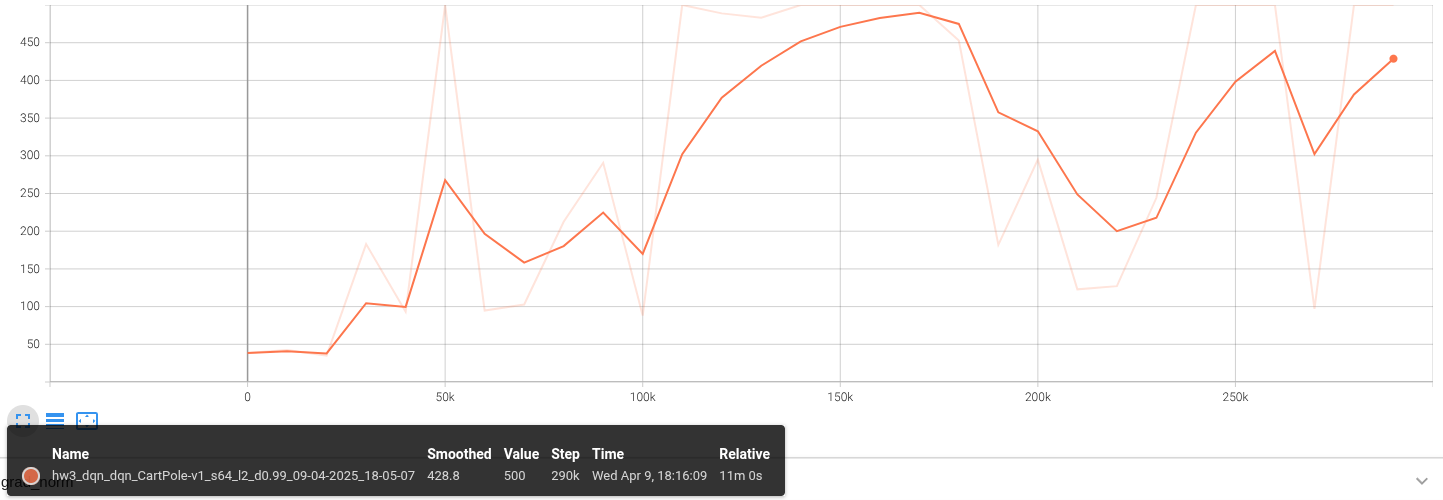
\includegraphics[width=0.8\textwidth]{imgs/hw3_dqn_CartPole_v1.png}
    \caption{Evaluation return on \texttt{CartPole-v1} with DQN.}
    \label{fig:cartpole}
\end{figure}

\begin{figure}[h]
  \centering
  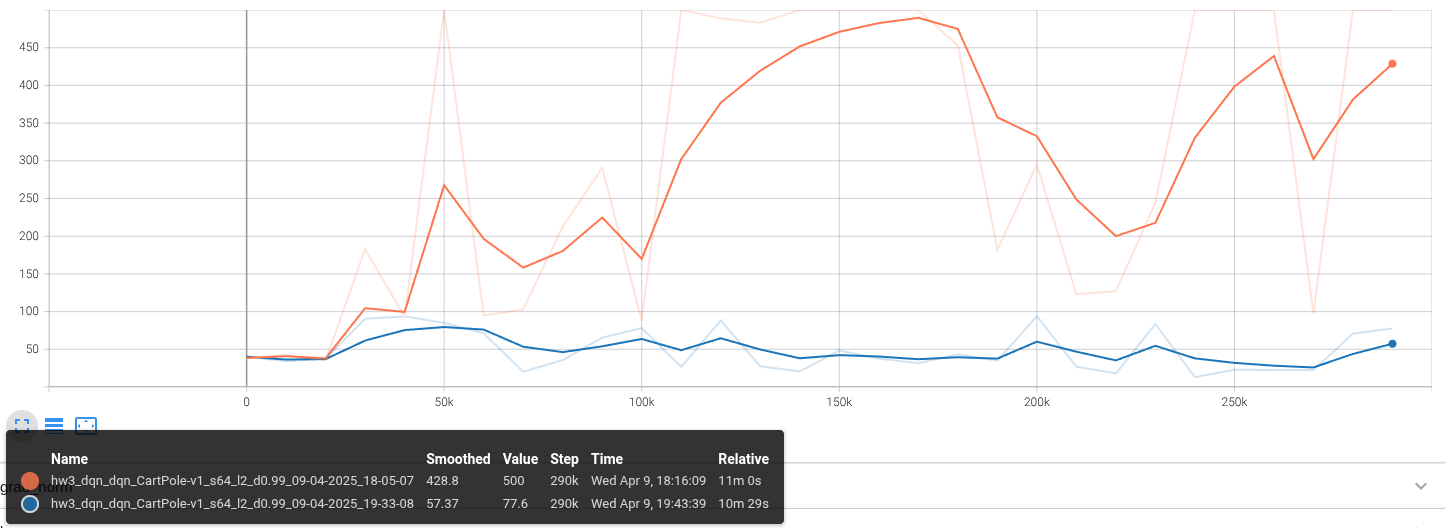
\includegraphics[width=0.8\textwidth]{imgs/hw3_dqn_CartPole_v1_lr005_eval_return.png}
  \caption{Evaluation return on \texttt{CartPole-v1} with \textcolor{blue}{DQN using lr 0.05}.}
  \label{fig:cartpole_high_lr}
\end{figure}

\begin{figure}[H]
  \centering
  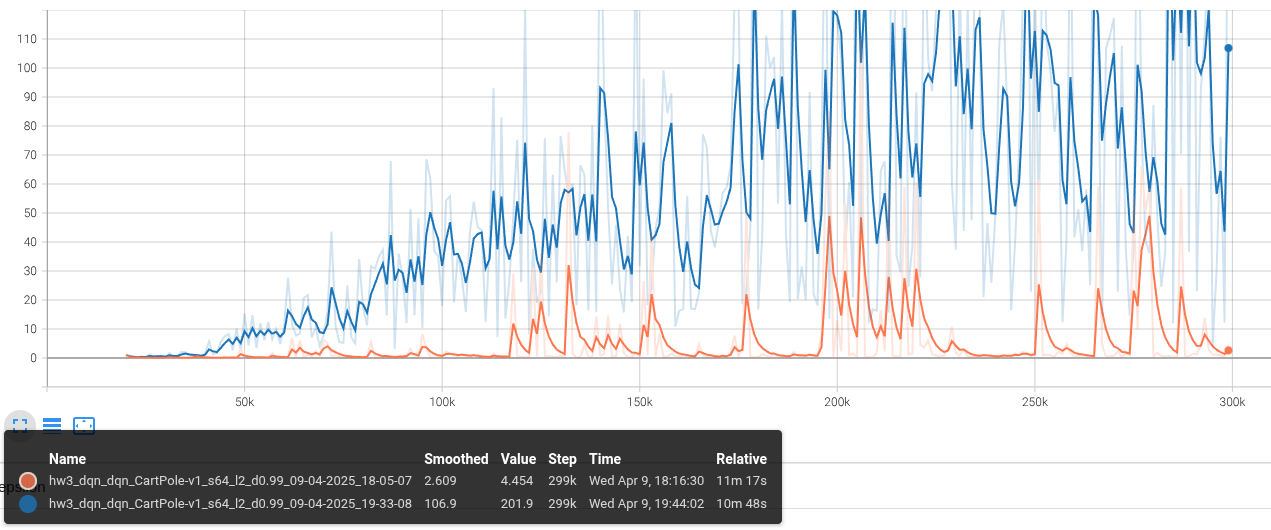
\includegraphics[width=0.49\linewidth]{imgs/hw3_dqn_CartPole_v1_lr005_critic_loss.png}
  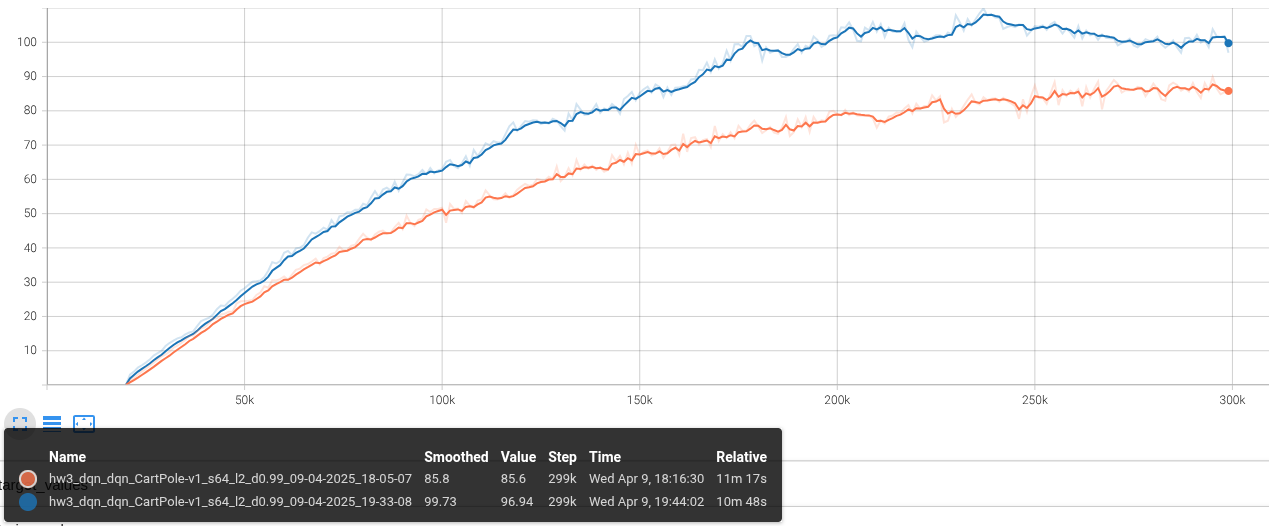
\includegraphics[width=0.49\linewidth]{imgs/hw3_dqn_CartPole_v1_lr005_q_values.png}
  \caption{Left: Critic loss, Right: Predicted Q-values on \texttt{CartPole-v1}. 
  \textcolor{blue}{\textbf{Blue}} corresponds to a high learning rate (\texttt{lr = 0.05}), while 
  \textcolor{orange}{\textbf{orange}} shows the default learning rate (\texttt{lr = 0.001}).}
  \label{fig:cartpole_high_lr_q_and_loss}
\end{figure}

\begin{tcolorbox}[answerbox, parbox=false]
  In \Cref{fig:cartpole_high_lr_q_and_loss}, we can see that the critic loss is much noisy and the predicted Q-values increase rapidly. This is because the learning rate is too high, causing the Q-values to oscillate and diverge. The critic loss also becomes unstable, leading to poor performance in the DQN.

  In DQN, the target for training is:
  \[y_t = r_t + \gamma \max_{a'} Q_{\text{target}} (s_{t+1},a')\]
  The loss is:
  \[\mathcal{L}=(Q(s_t,a_t)-y_t)^2\]
  With a high learning rate $\alpha$, gradient steps $\theta \leftarrow \theta - \alpha \nabla_\theta \mathcal{L}$ are very large, causing the Q-values to update too quickly. This can lead to divergence or oscillation.
\end{tcolorbox}

\subsection{Double Q-Learning}
Let's try to stabilize learning. The double-Q trick avoids overestimation bias in the critic update by using two different networks to \textit{select} the next action $a'$ and to \textit{estimate} its value:
\[a' = \textrm{arg}\max_{a'} Q_{\phi}(s', a')\]
\[Q_{\textrm{target}} = r + \gamma(1-d_t) Q_{\phi'}(s', a').\]
In our case, we'll keep using the target network $Q_{\phi'}$ to estimate the action's value, but we'll select the action using $Q_{\phi}$ (the online $Q$ network).

Implement this functionality in \verb|dqn_agent.py|.

\textbf{Deliverables}:
\begin{itemize}
    \item Run three more seeds of the lunar lander problem:

    You should expect a return of \textbf{200} by the end of training, and it should be fairly stable compared to your policy gradient methods from HW2.
    
    Plot returns from these three seeds in red, and the ``vanilla'' DQN results in blue, on the same set of axes. Compare the two, and describe in your own words what might cause this difference.

    \item Run your DQN implementation on the \verb|MsPacman-v0| problem. Our default configuration will use double-$Q$ learning by default. You are welcome to tune hyperparameters to get it to work better, but the default parameters should work (so if they don't, you likely have a bug in your implementation). Your implementation should receive a score of around \textbf{1500} by the end of training (1 million steps. \textbf{This problem will take about 3 hours with a GPU, or {\color{red} 6 hours} without, so start early!}

    \item Plot the average training return (\verb|train_return|) and eval return (\verb|eval_return|) on the same axes. You may notice that they look very different early in training! Explain the difference.
\end{itemize}

\begin{figure}[H]
  \centering
  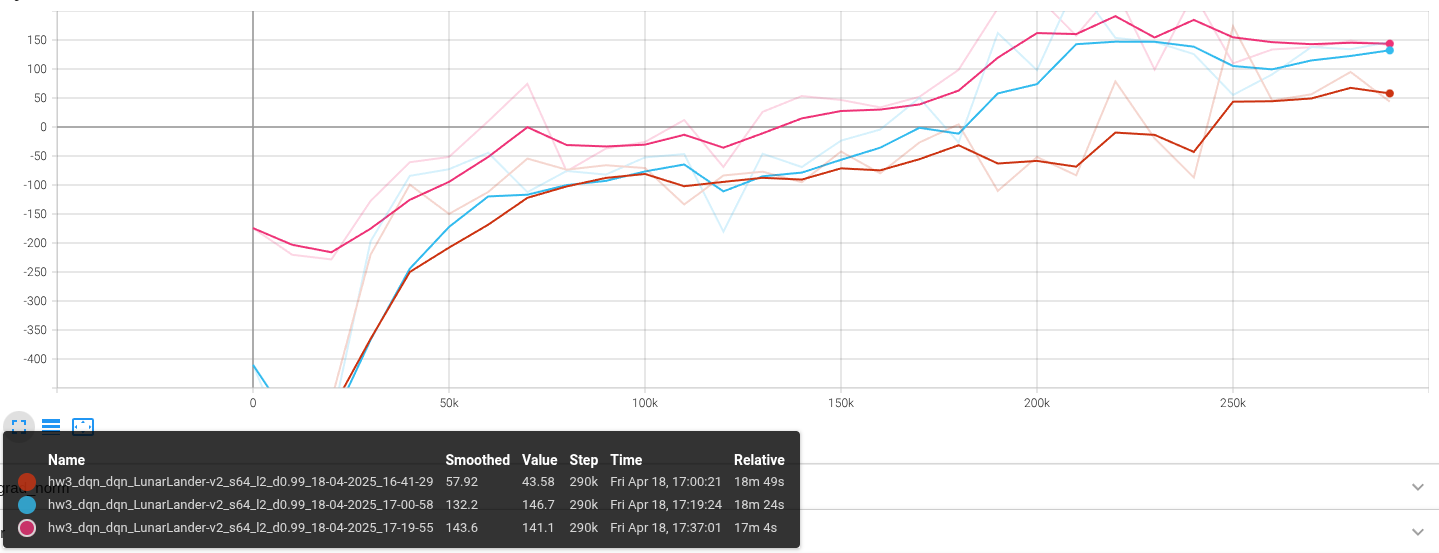
\includegraphics[width=0.49\linewidth]{imgs/hw3_dqn_LunarLander-v2.png}
  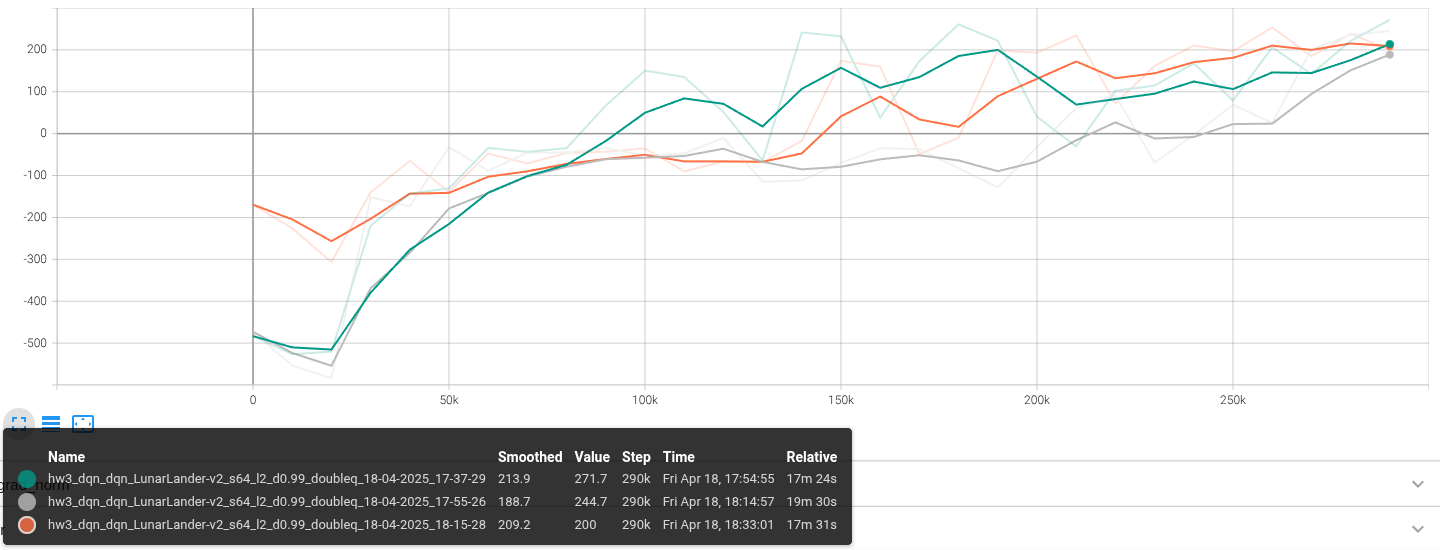
\includegraphics[width=0.49\linewidth]{imgs/hw3_double_dqn_LunarLander-v2.png}
  \caption{Left: DQN, Right: Double DQN on \texttt{LunarLander-v2}. Double DQN achieves around 200 return by the end of training.}
  \label{fig:lunarlander}
\end{figure}

\begin{figure}[H]
  \centering
  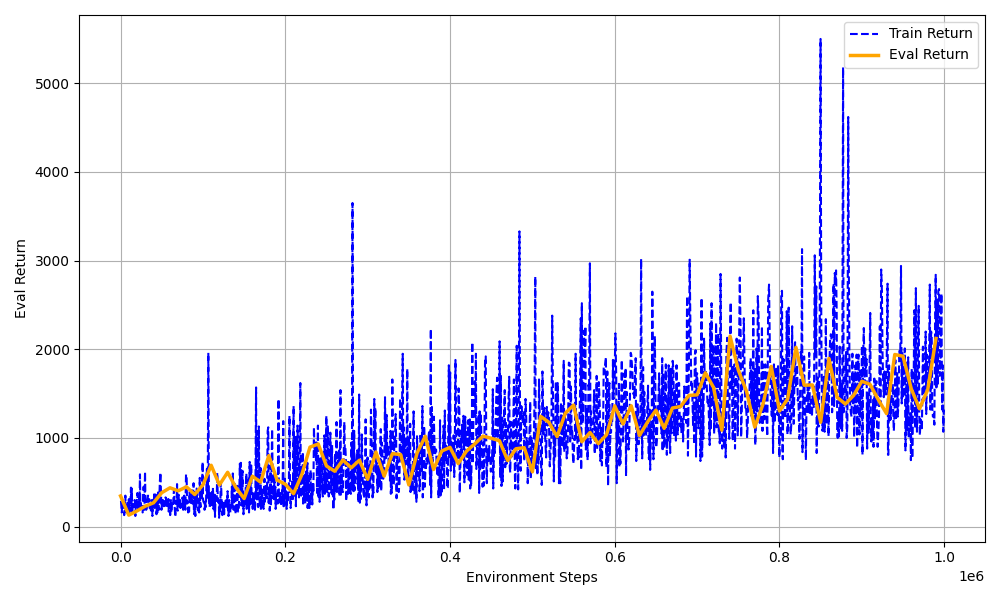
\includegraphics[width=0.8\linewidth]{imgs/hw3_double_dqn_MsPacman_Plotonce.png}
  \caption{The training return (\textcolor{blue}{blue}) and evaluation return (\textcolor{orange}{orange}) for the \texttt{MsPacman-v0} environment, both shown over 1 million steps. The evaluation return reaches above 1500 by the end of training.}
  \label{fig:double_dqn_mspacman}
\end{figure}

\subsection{Experimenting with Hyperparameters} Now let's analyze the sensitivity of Q-learning to hyperparameters. Choose one hyperparameter of your choice and run at least three other settings of this hyperparameter, in addition to the one used in Question 1, and plot all four values on the same graph. Your choice what you experiment with, but you should explain why you chose this hyperparameter in the caption. Create four config files in \verb|experiments/dqn/hyperparameters|, and look in \verb|cs285/env_configs/basic_dqn_config.py| to see which hyperparameters you're able to change. You can use any of the base YAML files as a reference.

Hyperparameter options could include:
\begin{itemize}
    \item Learning rate
    \item Network architecture
    \item Exploration schedule (or, if you'd like, you can implement an alternative to $\epsilon$-greedy)
\end{itemize}




\section{On-Policy Actor-Critic}
\subsection{Introduction}

DQN works well in discrete action spaces. In continuous action spaces, though, calculating target values requires maximizing $Q_{\phi'}(s', a')$ over \textit{all} values of $a'$!

Actor-critic methods are one way to deal with this limitation. In this framework, we have a \textit{parametrized} policy $\pi$ that gives us actions directly (rather than defining it implicitly by maximizing over $Q$-values). We can implement this in a very similar way to our policy gradient implementation from the previous homework:
\begin{align*}
\nabla_\theta J(\theta) &\approx \frac{1}{N} \sum_{i=1}^N \sum_{t=1}^T \nabla_\theta \log \pi_\theta(a_{it} | s_{it})\left(\left(\sum_{t'=t}^T \gamma^{t'-t} r(s_{it'}, a_{it'})\right) - V_\phi^\pi\left(s_{it}\right)\right).
\end{align*}

In this formulation, we estimate the Q function by taking the sum of rewards to go over each trajectory, and we subtract the value function baseline to obtain the advantage $$A^\pi(s_{t}, a_{t}) \approx \left(\sum_{t'=t}^T \gamma^{t'-t} r(s_{t'}, a_{t'})\right) - V_\phi^\pi\left(s_{t}\right)$$

In practice, the estimated advantage value suffers from high variance. Actor-critic addresses this issue by using a \textit{critic network} to estimate the sum of rewards to go. The most common type of critic network used is a value function, in which case our estimated advantage becomes
$$A^\pi(s_{t}, a_{t}) \approx r(s_{t}, a_{t}) + \gamma V_\phi^\pi\left(s_{t+1}\right) - V_\phi^\pi\left(s_{t}\right)$$
(Note that this also coincides with GAE with $\lambda = 0$.)

One additional consideration in actor-critic is updating the critic network itself. While we can use Monte Carlo rollouts to estimate the sum of rewards to go for updating the value function network (as we did in HW2), we can also \textit{bootstrap} our estimate by fitting it to the following \textit{target values}:
$$y_t = r(s_t, a_t) + \gamma V^\pi(s_{t+1})$$
we then regress onto these target values via the following regression objective which we can optimize with gradient descent:
$$\min_{\phi} \sum_{i,t} (V_{\phi}^\pi(s_{it}) - y_{it})^2$$
In theory, we need to perform this minimization every time we update our policy, so that our value function matches the behavior of the new policy. In practice however, this operation can be costly, so we may instead just take a few gradient steps at each iteration. Also note that since our target values are based on the old value function, we may need to recompute the targets with the updated value function, in the following fashion:
\begin{enumerate}
    \item Update targets with current value function
    \item Regress onto targets to update value function by taking a few gradient steps
    \item Redo steps 1 and 2 several times
\end{enumerate}
In all, the process of fitting the value function critic is an iterative process in which we go back and forth between computing target values and updating the value function to match the target values. Through experimentation, you will see that this iterative process is crucial for training the critic network.

\subsection{Implementation}

Your code will build off your solutions from homework 2. You will need to fill in the TODOS for the following parts of the code.

\begin{itemize}
    \item {\color{red} TODO}
\end{itemize}
 
\subsection{Evaluation}

Once you have a working implementation of actor-critic, you should prepare a report. The report should consist of figures for the question below. You should turn in the report as one PDF (same PDF as part 1) and a zip file with your code (same zip file as part 1). If your code requires special instructions or dependencies to run, please include these in a file called \verb+README+ inside the zip file.

\paragraph{Question 4: Sanity check with Pendulum-v1}
Now that you have implemented actor-critic, check that your solution works by running Cartpole-v0. \\
% \begin{lstlisting}[language=bash,breaklines=true]
% python cs285/scripts/run_hw3_actor_critic.py --env_name Pendulum-v1 -n 100 -b 1000 --exp_name q4_ac_1_1 -ntu 1 -ngsptu 1
% \end{lstlisting}
% In the example above, we alternate between performing one target update and one gradient update step for the critic. As you will see, this probably doesn't work, and you need to increase both the number of target updates and number of gradient updates. Compare the results for the following settings and report which worked best. Do this by plotting all the runs on a single plot and writing your takeaway in the caption.
% \begin{lstlisting}[language=bash,breaklines=true]
% python cs285/scripts/run_hw3_actor_critic.py --env_name CartPole-v0 -n 100 -b 1000 --exp_name q4_100_1 -ntu 100 -ngsptu 1
% \end{lstlisting}
% \begin{lstlisting}[language=bash,breaklines=true]
% python cs285/scripts/run_hw3_actor_critic.py --env_name CartPole-v0 -n 100 -b 1000 --exp_name q4_1_100 -ntu 1 -ngsptu 100
% \end{lstlisting}
% \begin{lstlisting}[language=bash,breaklines=true]
% python cs285/scripts/run_hw3_actor_critic.py --env_name CartPole-v0 -n 100 -b 1000 --exp_name q4_10_10 -ntu 10 -ngsptu 10
% \end{lstlisting}
At the end, the best setting from above should match the policy gradient results from Cartpole in hw2 (200).

\paragraph{Question 5: Run actor-critic with more difficult tasks}
Use the best setting from the previous question to run InvertedPendulum and HalfCheetah:
% \begin{lstlisting}[language=bash,breaklines=true]
% python cs285/scripts/run_hw3_actor_critic.py --env_name InvertedPendulum-v4 --ep_len 1000 --discount 0.95 -n 100 -l 2 -s 64 -b 5000 -lr 0.01 --exp_name q5_<ntu>_<ngsptu> -ntu <> -ngsptu <>
% \end{lstlisting}
where \texttt{<ntu>\_<ngsptu>} is replaced with the parameters you chose.


Your results should roughly match those of policy gradient.
After 150 iterations, your HalfCheetah return should be around 150.
After 100 iterations, your InvertedPendulum return should be around 1000.
Your deliverables for this section are plots with the eval returns for both enviornments.

As a debugging tip, the returns should start going up immediately.
For example, after 20 iterations, your HalfCheetah return should be above -40 and your InvertedPendulum return should near or above 100.
However, there is some variance between runs, so the 150-iteration (for HalfCheetah) and 100-iteration (for InvertedPendulum) results are the numbers we use to grade.






\paragraph{SAC-related questions.} 
We wanted to address some of the common questions that have been asked regarding Question 6 of the HW. The full algorithm for SAC is summarized below, the equations listed in this paper will be helpful for you: {\url{https://arxiv.org/pdf/1812.05905}}. Some definitions that will be useful:
\begin{enumerate}
    \item What is alpha and how to update it: Alpha is the entropy regularization coefficient denoting how much exploration to add to the policy. You should update based on Eq. 18 in Section 5 in the above paper as follows: 
    $$
    J(\alpha)=\mathop{\mathbb{E}}_{a_t \sim \pi_t}[-\alpha\log_{\pi_t}(a_t|s_t) - \alpha\bar{\mathcal{H}}].
    $$
    \item Target entropy is the negative of the action space dimension that is used to update the alpha term.
    \item SquashedNorm: This is a function that takes in mean and std as in previous homeworks, and will give you a distribution that you can sample your action from. 
    \item To update the critic, refer to how to update Q-function parameters in Equation 6 of the paper above as follows: \\
    $$J_{Q}(\theta) = Q_{\theta}(s_t, a_t) - (r(s_t, a_t) + \gamma (Q_{\bar{\theta}}(s_{t+1}, a_{t+1}) - \alpha \log(\pi_{\phi}(a_{t+1}, s_{t+1})))$$
    \item To update the policy, follow Equation 18: \\
    $$J(\alpha) = E_{a_t \sim \pi_t} [- \alpha \log \pi_{t}(a_t|s_t) - \alpha \bar{\mathcal{H}}]$$
    \item You don't need to alter any parameters from the SAC run commands. The correct implementation should work with the provided default parameters.
    
\end{enumerate}


\end{document}